\documentclass{article}

\usepackage{graphicx}
\usepackage{tikz}
\usepackage{tikzsymbols}
\usetikzlibrary{calc,patterns,shapes.geometric}
\pagestyle{empty}
\usepackage[margin=0pt]{geometry}
\geometry{papersize={14in,12in}}

\def\centerarc[#1](#2)(#3:#4:#5){\draw[#1] ($(#2)+({#5*cos(#3)},{#5*sin(#3)})$) arc (#3:#4:#5);}

\begin{document}
	\begin{figure}
		\centering
		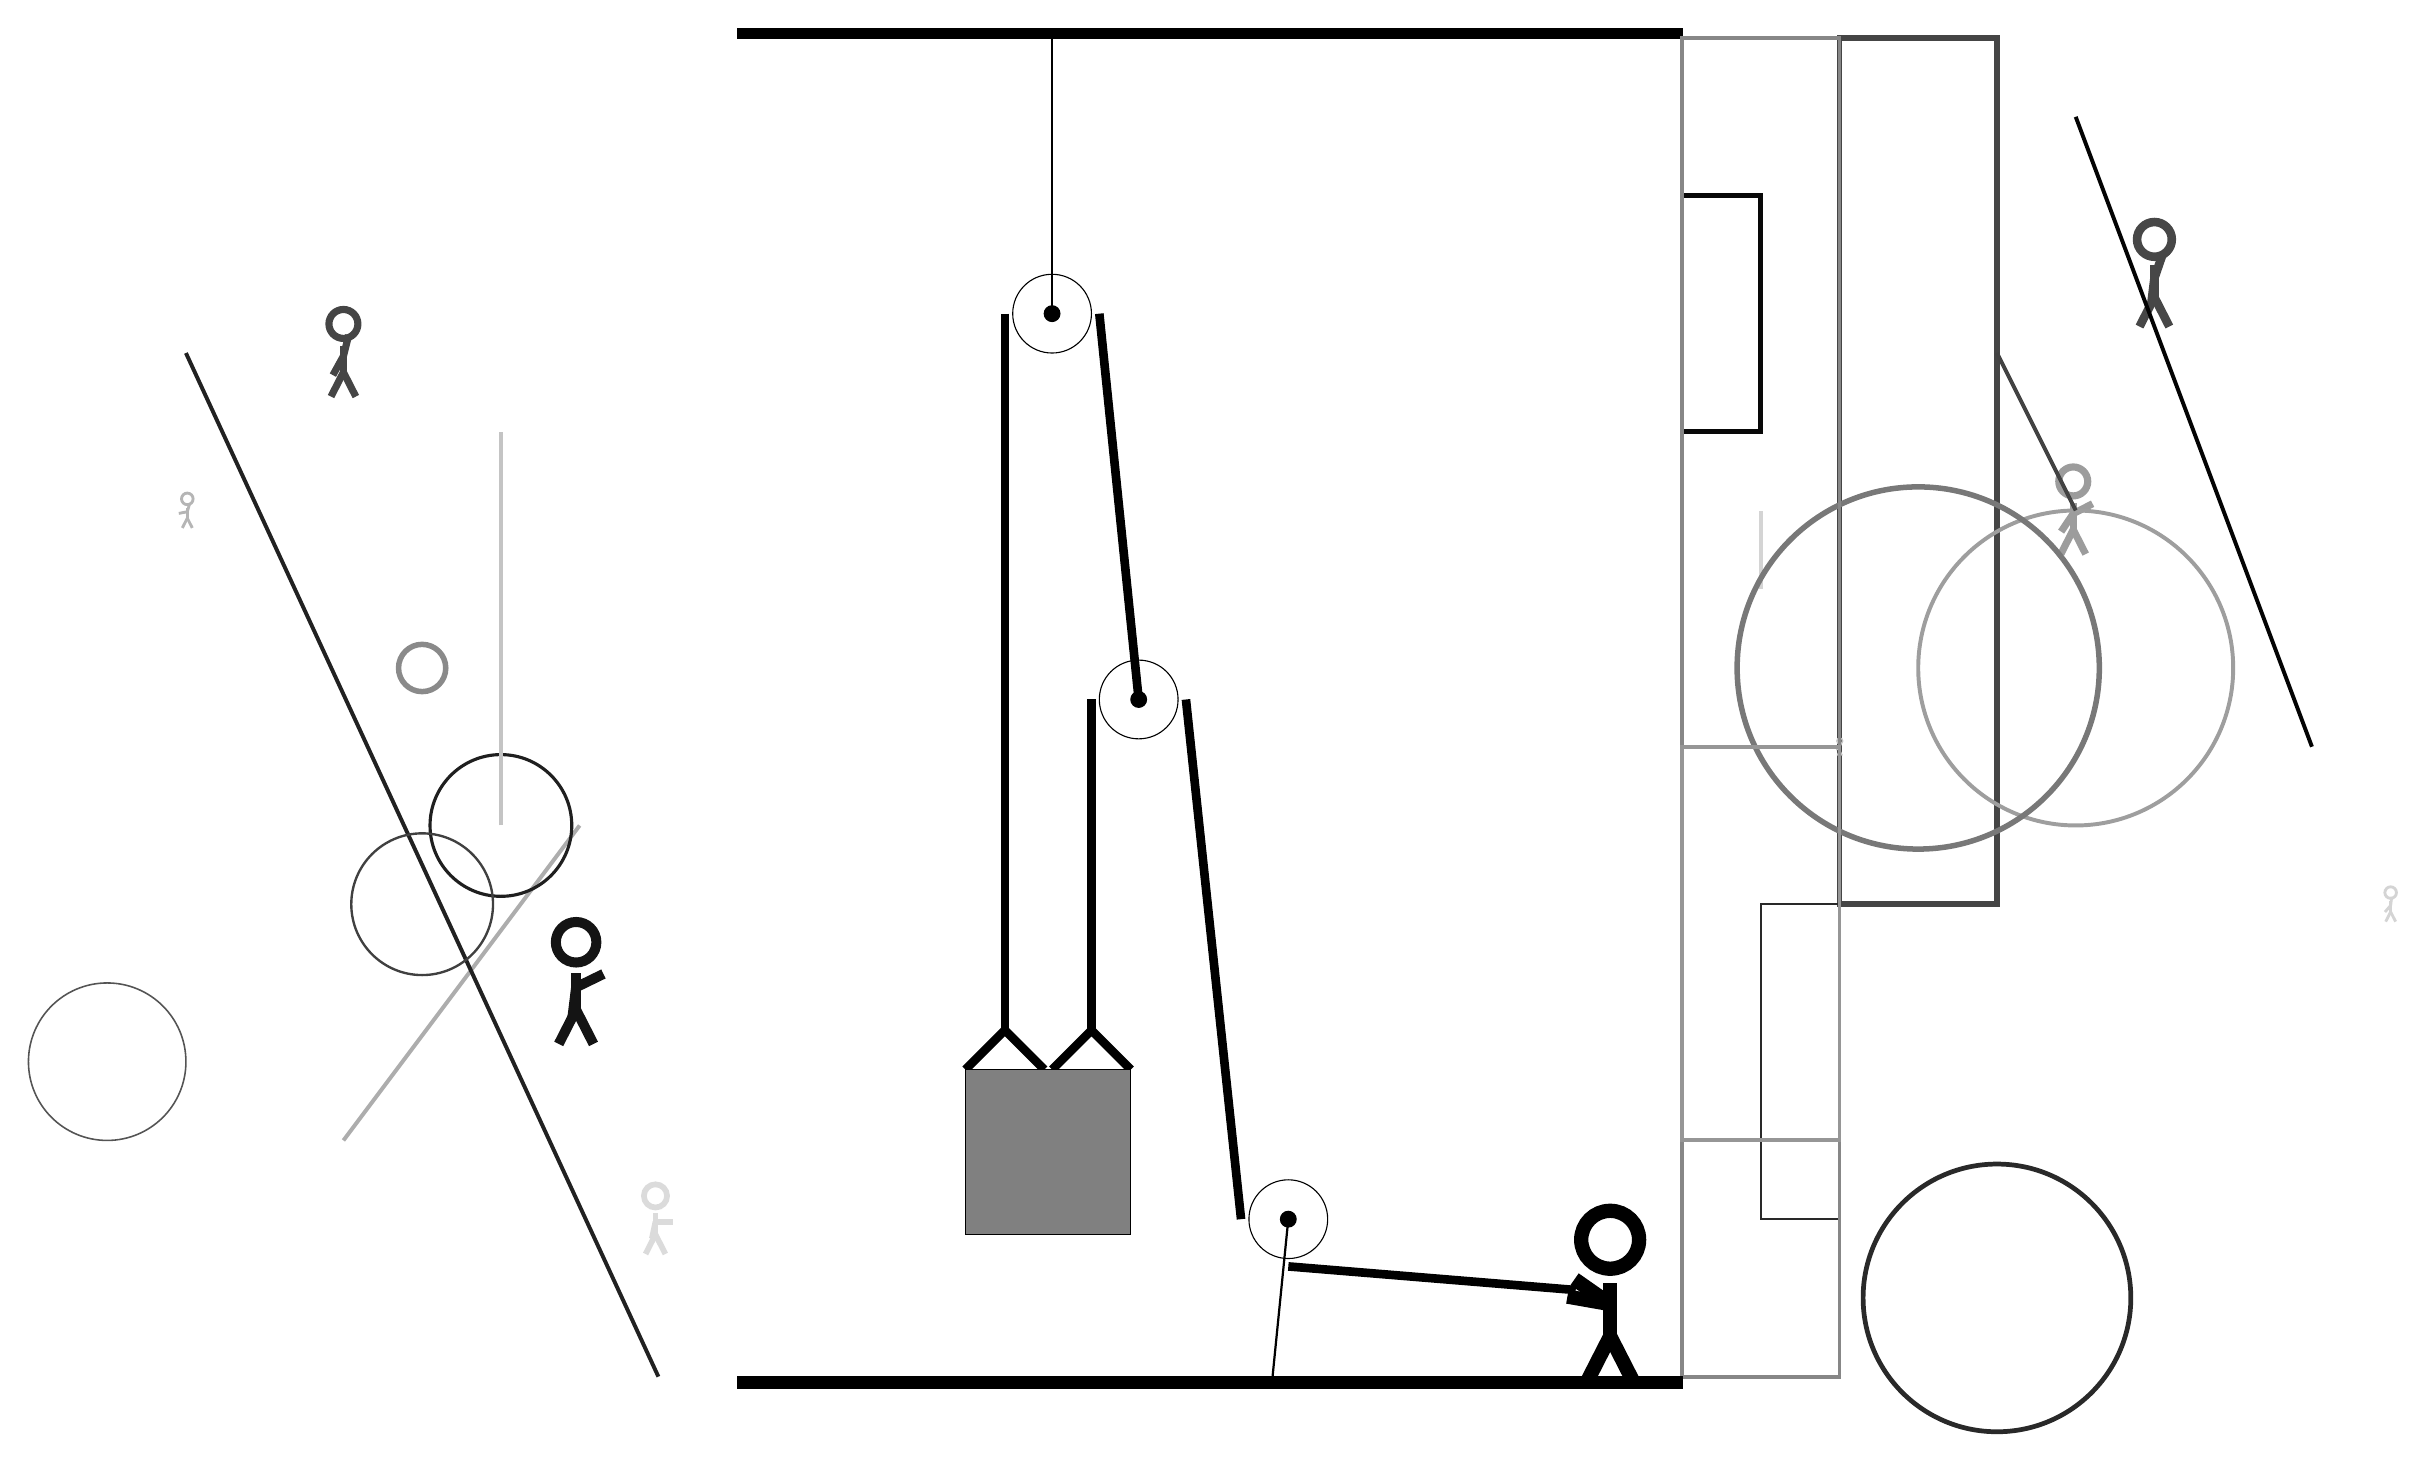
\begin{tikzpicture}
			%%%%% START %%%%%
			
			\draw[fill=black] (-2, 14) rectangle (10, 14.125);
			
			\draw (2, 10.5) circle (0.5);
			\draw[fill=black] (2, 10.5) circle (0.1);
			\draw[thick] (2, 10.5) -- (2, 14);
			
			\draw (3.1, 5.6) circle (0.5);
			\draw[fill=black] (3.1, 5.6) circle (0.1);
			
			\draw (5, -1) circle (0.5);
			\draw[fill=black] (5, -1) circle (0.1);
			\draw[thick] (5, -1) -- (4.8, -3);
			
			\draw[line width = 1.1mm]  (0.9, 0.9) -- (1.4, 1.4) -- (1.9, 0.9);
			\draw[line width = 1.1mm]  (2.0, 0.9) -- (2.5, 1.4) -- (3.0, 0.9);
			\draw[fill=black!50] (0.9, 0.9) rectangle (3.0, -1.2);
			
			\draw[line width = 1.1mm] (1.4, 10.5) -- (1.4, 1.4);
			\centerarc[line width = 1.1mm](2, 10.5)(0:180:0.6);
			\draw[line width = 1.1mm] (2.6, 10.5) -- (3.1, 5.6);
			\draw[line width = 1.1mm] (2.5, 5.6) -- (2.5, 1.4);
			\centerarc[line width = 1.1mm](3.1, 5.6)(0:180:0.6);
			\draw[line width = 1.1mm] (3.7, 5.6) -- (4.4, -1);
			\centerarc[line width = 1.1mm](5, -1)(180:270:0.6);
			\draw[line width = 1.1mm] (5, -1.6) -- (8.65, -1.9);
			
			\node[line width=0.5mm, color=black!17] at (19, 3) {\Strichmaxerl[2][49][83]};
			
			\draw[line width=0.7mm, color=black!73] (12, 14) rectangle (14, 3);
			\draw [line width=0.2mm, color=black!67](-10, 1) circle (1.0);
			\draw[line width=0.5mm, color=black!32](-4, 4) -- (-7, 0);
			\draw[line width=0.5mm, color=black!17](11, 7) -- (11, 8);
			
			\node[line width=0.5mm, color=black!72] at (16, 11) {\Strichmaxerl[6][83][71]};
			\node[line width=0.3mm, color=black!23] at (12, 5) {\Strichmaxerl[1][38][68]};
			\node[line width=0.5mm, color=black!39] at (15, 8) {\Strichmaxerl[5][56][27]};
			\node[line width=0.5mm, color=black!92] at (-4, 2) {\Strichmaxerl[7][83][26]};
			
			\draw[line width=0.5mm, color=black!87](-3, -3) -- (-9, 10);
			
			\draw [line width=0.6mm, color=black!84](14, -2) circle (1.7);
			\draw [line width=0.5mm, color=black!38](15, 6) circle (2.0);
			\draw[line width=0.5mm, color=black!74](15, 8) -- (14, 10);
			\draw[line width=0.6mm, color=black!97] (10, 12) rectangle (11, 9);
			\draw [line width=0.4mm, color=black!88](-5, 4) circle (0.9);
			\draw [line width=0.7mm, color=black!53](13, 6) circle (2.3);
			\draw[line width=0.3mm, color=black!84] (11, -1) rectangle (12, 3);
			
			\node[line width=0.5mm, color=black!14] at (-3, -1) {\Strichmaxerl[4][78][0]};
			\draw[line width=0.5mm, color=black!47] (12, -3) rectangle (10, 14);
			
			\draw[line width=0.5mm, color=black!41] (12, 5) rectangle (10, 0);
			\draw[line width=0.5mm, color=black!99](15, 13) -- (18, 5);
			
			\draw [line width=0.3mm, color=black!75](-6, 3) circle (0.9);
			\node[line width=0.7mm, color=black!29] at (-9, 8) {\Strichmaxerl[2][11][74]};
			\node[line width=0.4mm, color=black!73] at (-7, 10) {\Strichmaxerl[5][61][76]};
			\draw[line width=0.5mm, color=black!23](-5, 4) -- (-5, 9);
			
			\draw [line width=0.7mm, color=black!46](-6, 6) circle (0.3);
			
			
			\node at (9, -2) {\Strichmaxerl[10][-35][170]};
			
			\draw[fill=black] (-2, -3) rectangle (10, -3.15);
			
			%%%%% END %%%%%
		\end{tikzpicture}
	\end{figure}	
\end{document}